\documentclass{standalone}
\usepackage{tikz}
\usetikzlibrary{patterns, positioning}

\begin{document}
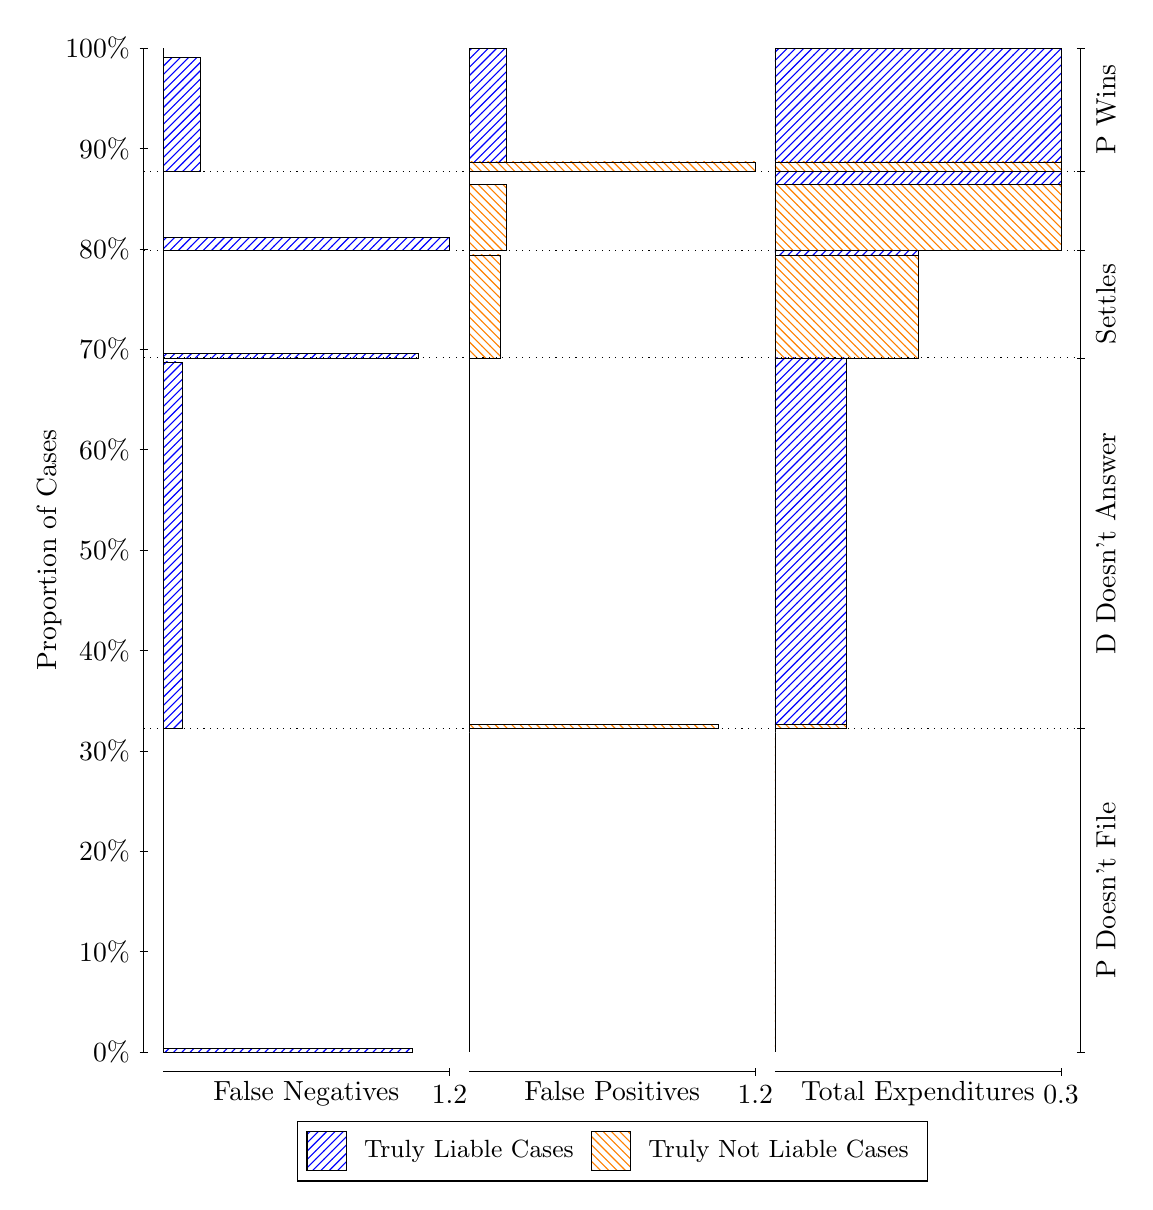
\begin{tikzpicture}
\draw[black, very thin] (1.5,1.75) -- (1.5,14.5);
\node[rotate=90, anchor=center] at (0.3, 8.125) {Proportion of Cases};
\draw[black, very thin] (1.45,1.75) -- (1.55,1.75);
\node[anchor=east] at (1.45, 1.75) {0\%};
\draw[black, very thin] (1.45,3.025) -- (1.55,3.025);
\node[anchor=east] at (1.45, 3.025) {10\%};
\draw[black, very thin] (1.45,4.3) -- (1.55,4.3);
\node[anchor=east] at (1.45, 4.3) {20\%};
\draw[black, very thin] (1.45,5.575) -- (1.55,5.575);
\node[anchor=east] at (1.45, 5.575) {30\%};
\draw[black, very thin] (1.45,6.85) -- (1.55,6.85);
\node[anchor=east] at (1.45, 6.85) {40\%};
\draw[black, very thin] (1.45,8.125) -- (1.55,8.125);
\node[anchor=east] at (1.45, 8.125) {50\%};
\draw[black, very thin] (1.45,9.4) -- (1.55,9.4);
\node[anchor=east] at (1.45, 9.4) {60\%};
\draw[black, very thin] (1.45,10.675) -- (1.55,10.675);
\node[anchor=east] at (1.45, 10.675) {70\%};
\draw[black, very thin] (1.45,11.95) -- (1.55,11.95);
\node[anchor=east] at (1.45, 11.95) {80\%};
\draw[black, very thin] (1.45,13.225) -- (1.55,13.225);
\node[anchor=east] at (1.45, 13.225) {90\%};
\draw[black, very thin] (1.45,14.5) -- (1.55,14.5);
\node[anchor=east] at (1.45, 14.5) {100\%};

\draw[black, very thin] (13.4,1.75) -- (13.4,14.5);
\draw[black, very thin] (13.35,1.75) -- (13.45,1.75);
\node[anchor=west] at (13.35, 1.75) {};
\draw[black, very thin] (13.35,5.8555) -- (13.45,5.8555);
\node[anchor=west] at (13.35, 5.8555) {};
\draw[black, very thin] (13.35,10.566) -- (13.45,10.566);
\node[anchor=west] at (13.35, 10.566) {};
\draw[black, very thin] (13.35,11.932) -- (13.45,11.932);
\node[anchor=west] at (13.35, 11.932) {};
\draw[black, very thin] (13.35,12.934) -- (13.45,12.934);
\node[anchor=west] at (13.35, 12.934) {};
\draw[black, very thin] (13.35,14.5) -- (13.45,14.5);
\node[anchor=west] at (13.35, 14.5) {};

\draw[black, very thin, pattern color=blue, pattern=north east lines] (1.75,1.75) rectangle (4.9094,1.7975);
\draw[black, very thin, pattern color=orange, pattern=north west lines] (1.75,1.7975) rectangle (1.75,5.8555);
\draw[black, very thin, pattern color=blue, pattern=north east lines] (1.75,5.8555) rectangle (1.987,10.513);
\draw[black, very thin, pattern color=orange, pattern=north west lines] (1.75,10.513) rectangle (1.75,10.566);
\draw[black, very thin, pattern color=blue, pattern=north east lines] (1.75,10.566) rectangle (4.9884,10.624);
\draw[black, very thin, pattern color=orange, pattern=north west lines] (1.75,10.624) rectangle (1.75,11.932);
\draw[black, very thin, pattern color=blue, pattern=north east lines] (1.75,11.932) rectangle (5.3833,12.099);
\draw[black, very thin, pattern color=orange, pattern=north west lines] (1.75,12.099) rectangle (1.75,12.934);
\draw[black, very thin, pattern color=blue, pattern=north east lines] (1.75,12.934) rectangle (2.2239,14.379);
\draw[black, very thin, pattern color=orange, pattern=north west lines] (1.75,14.379) rectangle (1.75,14.5);
\draw[black, very thin, pattern color=orange, pattern=north west lines] (5.6333,1.75) rectangle (5.6333,5.808);
\draw[black, very thin, pattern color=blue, pattern=north east lines] (5.6333,5.808) rectangle (5.6333,5.8555);
\draw[black, very thin, pattern color=orange, pattern=north west lines] (5.6333,5.8555) rectangle (8.7928,5.9089);
\draw[black, very thin, pattern color=blue, pattern=north east lines] (5.6333,5.9089) rectangle (5.6333,10.566);
\draw[black, very thin, pattern color=orange, pattern=north west lines] (5.6333,10.566) rectangle (6.0283,11.873);
\draw[black, very thin, pattern color=blue, pattern=north east lines] (5.6333,11.873) rectangle (5.6333,11.932);
\draw[black, very thin, pattern color=orange, pattern=north west lines] (5.6333,11.932) rectangle (6.1072,12.767);
\draw[black, very thin, pattern color=blue, pattern=north east lines] (5.6333,12.767) rectangle (5.6333,12.934);
\draw[black, very thin, pattern color=orange, pattern=north west lines] (5.6333,12.934) rectangle (9.2667,13.055);
\draw[black, very thin, pattern color=blue, pattern=north east lines] (5.6333,13.055) rectangle (6.1072,14.5);
\draw[black, very thin, pattern color=orange, pattern=north west lines] (9.5167,1.75) rectangle (9.5167,5.808);
\draw[black, very thin, pattern color=blue, pattern=north east lines] (9.5167,5.808) rectangle (9.5167,5.8555);
\draw[black, very thin, pattern color=orange, pattern=north west lines] (9.5167,5.8555) rectangle (10.425,5.9089);
\draw[black, very thin, pattern color=blue, pattern=north east lines] (9.5167,5.9089) rectangle (10.425,10.566);
\draw[black, very thin, pattern color=orange, pattern=north west lines] (9.5167,10.566) rectangle (11.333,11.873);
\draw[black, very thin, pattern color=blue, pattern=north east lines] (9.5167,11.873) rectangle (11.333,11.932);
\draw[black, very thin, pattern color=orange, pattern=north west lines] (9.5167,11.932) rectangle (13.15,12.767);
\draw[black, very thin, pattern color=blue, pattern=north east lines] (9.5167,12.767) rectangle (13.15,12.934);
\draw[black, very thin, pattern color=orange, pattern=north west lines] (9.5167,12.934) rectangle (13.15,13.055);
\draw[black, very thin, pattern color=blue, pattern=north east lines] (9.5167,13.055) rectangle (13.15,14.5);
\draw[black, dotted] (1.5,5.8555) -- (13.4,5.8555);
\draw[black, dotted] (1.5,10.566) -- (13.4,10.566);
\draw[black, dotted] (1.5,11.932) -- (13.4,11.932);
\draw[black, dotted] (1.5,12.934) -- (13.4,12.934);
\draw[black, very thin] (1.75,1.5) -- (5.3833,1.5);
\node[anchor=north] at (3.5667, 1.5) {False Negatives};
\draw[black, very thin] (5.3833,1.45) -- (5.3833,1.55);
\node[anchor=north] at (5.3833, 1.45) {1.2};

\draw[black, very thin] (5.6333,1.5) -- (9.2667,1.5);
\node[anchor=north] at (7.45, 1.5) {False Positives};
\draw[black, very thin] (9.2667,1.45) -- (9.2667,1.55);
\node[anchor=north] at (9.2667, 1.45) {1.2};

\draw[black, very thin] (9.5167,1.5) -- (13.15,1.5);
\node[anchor=north] at (11.333, 1.5) {Total Expenditures};
\draw[black, very thin] (13.15,1.45) -- (13.15,1.55);
\node[anchor=north] at (13.15, 1.45) {0.3};

\node[black, centered, rotate=90] at (13.72, 3.8027) {P Doesn't File};
\node[black, centered, rotate=90] at (13.72, 8.2107) {D Doesn't Answer};
\node[black, centered, rotate=90] at (13.72, 11.249) {Settles};

\node[black, centered, rotate=90] at (13.72, 13.717) {P Wins};

\draw (7.449999999999999,1.5) node[draw=none] (baseCoordinate) {};
\begin{scope}[align=center]
        \matrix[scale=0.5, draw=black, below=0.5cm of baseCoordinate, nodes={draw}, column sep=0.1cm]{
            \node[rectangle, draw, minimum width=0.5cm, minimum height=0.5cm, pattern=north east lines, pattern color=blue] {}; &
            \node[draw=none, font=\small] (B) {Truly Liable Cases}; &
            \node[rectangle, draw, minimum width=0.5cm, minimum height=0.5cm, pattern=north west lines, pattern color=orange] {}; &
            \node[draw=none, font=\small] (B) {Truly Not Liable Cases}; \\
            };
\end{scope}

\end{tikzpicture}
\end{document}